\section{Power Model Generator}
\label{sec:main}
\subsection{Linear Power Model}

To obtain power numbers from FPGA simulation, power model generator provides the linear power model of the target design.
Figure \ref{fig:model} shows the graphical representation of the linear power model.
The power model generator solves the linear equation $y = Ac$, 
where $y = [y_1 \ y_2 \ ... \ y_T]$ is the gate-level power consumption at cycle t
and $A = [x_1 \ x_2 \ ... \ x_T]$ is a transition matrix of the target design.
To solve this equation, we take advantage of linear regression with the LMS algorithm.
The solution $c$ of the system is later multiplied by signal activities for power analysis.

\begin{figure}
  \centering
  \resizebox{0.3\columnwidth}{!}{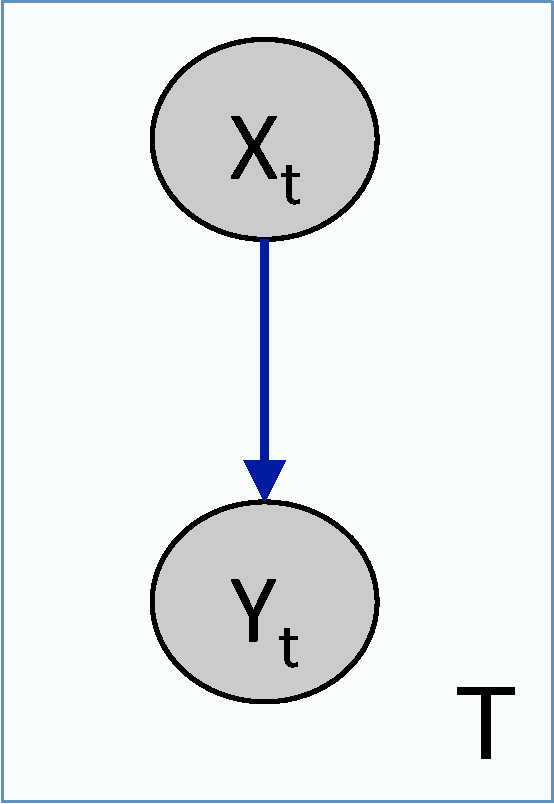
\includegraphics{figure/model}}
  \caption{Graphical representation of the linear power model}
  \label{fig:model}
\end{figure}

In our methodology, the signal activities are provided by FPGA simulation.
Thus, if we have the power model from the target design's microbenchmarks and the signal activities for applications,
we can analyze the power consumption of the specific applications.
Note that FPGA simulation can provide the signal activities much faster than the gate-level simulation or 
cycle-accurate software simulators.

\subsection{LMS Algorithm with Cost Function}

One problem of the linear power model is FPGA simulation cannot provide the switching activities for all the signals.
This is mainly because adding counters for all the signals complicates the original design. 
Thus, we need to pick the signals to be watched during FPGA simulation.

\begin{algorithm}
  \caption{\emph{Take N steps}}
  \begin{algorithmic}[1]
	\STATE Set $f(i) = 0$ and $c^{(0)} = 0$
	\REPEAT
		\STATE Update $f(i) = f(i) + [(c^{(l)})_i * (x_t)_i]$
		\STATE Update $c^{(l+1)} = c^{(l)} + \rho(y_t - c^{(t)T}x_t)$
	\UNTIL{$c^{(l)}$ converges}
  \end{algorithmic}
  \label{alg:lms}
\end{algorithm}

Our approach is to assign cost function to the signals when executing the LMS algorithm.
Algorithm \ref{alg:lms} shows the LMS algorithm with the cost function.

Let $f(i)$ be the cost function for signal $i$. For each iteration of the LMS algorithm,
$f(i)$ is updated according to the current parameter value $c^{(l)}$ and the current i's transition 
in the vector $x_t$. Thus, the cost function means 
the sum of the signal's contribution to each iteration's mean value estimation.
We select the signals with the highest cost function values.

